\subsection{Time complexity and performance}
%We are interested in knowing which element type among state, transition and event dominates the running time of the reverse engineering in case of creating new SM from code. 
To analyze the time complexity, we consider two tasks: semantic verification and SM construction from the verification output. 
%Let us use the following parameters of the input SM used in code generation: $n_{s}$ = number of states, $n_{t}$ = number of transitions, $n_{ce}$ = number of call events, $n_{te}$ = number of time events, $n_{a}$ = number of actions and guards including entry/exit/transition actions and guards which are all implemented in the context class. 

For each state, the semantic verification consists of the following phases: (1) detecting composite/sub-state pattern, (2) loop over all methods of a state class, (3) detecting entry action pattern, (4) detecting exit action pattern, (5) detecting processing \ti{CallEvent}, (6) detecting processing \ti{TimeEvent}, and (7) detecting default state pattern. 
\begin{comment}
\begin{itemize}
  \item Detecting composite/sub-state pattern: $C_{childParentPattern} = ns^2 = O (ns^2)$.
  \item Loop over all methods of a state class: $CfindAllStateOperation = ns + nce + nt$. 
  \item Detecting entry action pattern: $Centry = na + CverifyTransition + CfindFunctionDefinition 
      = 6ns + 6nce + 5na + nt$
   \item Detecting exit action pattern: Cexit = 3nce + 3ns + 3na + nt
   \item Detecting processing CallEvent: CprocessEvent = 7nce + 6ns + 2nt + 2na 
   \item Detecting processing TimeEvent: CprocessTimeEvent = 6nce + 6ns + 2nt + 2na
   \item Detecting default state pattern: CsetInitDefaultState = 3nce + 3ns + nt + na
\end{itemize}

\begin{itemize}
  \item Detecting composite/sub-state pattern
  \item Loop over all methods of a state class
  \item Detecting entry action pattern
   \item Detecting exit action pattern
   \item Detecting processing \ti{CallEvent}
   \item Detecting processing \ti{TimeEvent}
   \item Detecting default state pattern
\end{itemize}
\end{comment}

Due to the space limitation, we cannot present the detail of the complexity of each phase. To sum up, the semantic verification has a worst-case complexity (abbreviations $n_{s}$, $n_{t}$, $n_{ce}$, $n_{a}$ are the number of states, transitions, call events and actions, respectively) $C_{1} = n_{s}(n_{s^2} + 9n_{t^2} + 6n_{t}n_{s} + 2n_{a}n_{ce}) = O (n_{s^3}) + O (n_{t}n_{s^2}) + O (n_{s}n_{t^2}) = O (n^3)$ with $n = max (n_{t}, n_{s})$. The worst-case occurs if a state can accept all incoming events, all transitions have the same source state and all states contain each other. This case is unrealistic.

The SM construction from the verification output has a worst-case time complexity $C_{2} = O (n_{s^2}) + O (n_{s} n_{t}) = O (n_{^2})$. Therefore, the reverse engineering has a worst-case complexity of $O (n^3)$ with $n = max (n_{s}, n_{t})$.

To analyze the performance of reverse engineering, we randomly generate 5 models with base set up information in which the numbers of states and transitions are 20 and 50, respectively. We use a Dell Latitude E554 laptop with a 2.1GHz Intel Core i7 with 16 Gb of RAM. The running time of the reverse for the generated code associated with these models is measured. To analyze the impact of state and transition to the reverse performance, 
%we change the set up information by increasing either the number of states or transitions, and keep intact the other. 
we increase the number of states and transitions by five, alternatively. The models resulting from the increase are used for generating code. The running time of reverse engineering the new generated code is measured. For each measurement, three times are computed, the median of these measured values are retained. 

\begin{comment}
\begin{table}
\centering
\caption{Time measurements}
\label{table:time-measurment}
\begin{tabular}{|l|l|l|}
\hline
\rowcolor{Gray}
Increase of the number of instances  & State  & Transition \\ \hline
5            & 78021  & 62271      \\ \hline
10           & 83025  & 68374      \\ \hline
15           & 96761  & 64176      \\ \hline
20           & 118879 & 71728      \\ \hline
25           & 132763 & 73445      \\ \hline
%30           & 153120 & 75314      \\ \hline
%35           & 163538 & 78647      \\ \hline
%40           & 185361 & 81547      \\ \hline
\end{tabular}
\end{table}
\end{comment}

%Table \ref{table:time-measurment} shows the increase of the number of instances for states and transitions, and the execution time in millisecond for reversing the resulting models obtained by increasing the number of instances. 
Fig. \ref{fig:graph} shows the increase of the number of instances for states and transitions, and the increase time rate, which is the execution time for reversing modified models divided by the execution time for reversing the original model. The median execution time for reversing the original model is 64557 ms. The results show that the number of states has a higher performance impact than the number of transitions. %Fig. \ref{fig:graph} (the increase time rate is the execution time for reversing modified models divided by the execution time for reversing the original model) shows the performance comparison between the execution time for reversing the original model and the models modified by adding states and transitions. 
When the number of added states grows, the running time for reverse also grows quickly. Whereas, in case of transitions, the difference is small and not clear as we analyze that the worst-case complexity never occurs.

%Fig. \ref{fig:graph} (the increase time rate is the execution time for reversing modified models divided by the execution time for reversing the original model) also shows the performance comparison between the execution time for reversing the original model and the models modified by adding states and transitions. When the number of added states grows, the running time for reverse also grows quickly. Whereas, in case of transitions, the difference is small and not clear as we analyze that the worst-case complexity never occurs.

\begin{figure}
\centering
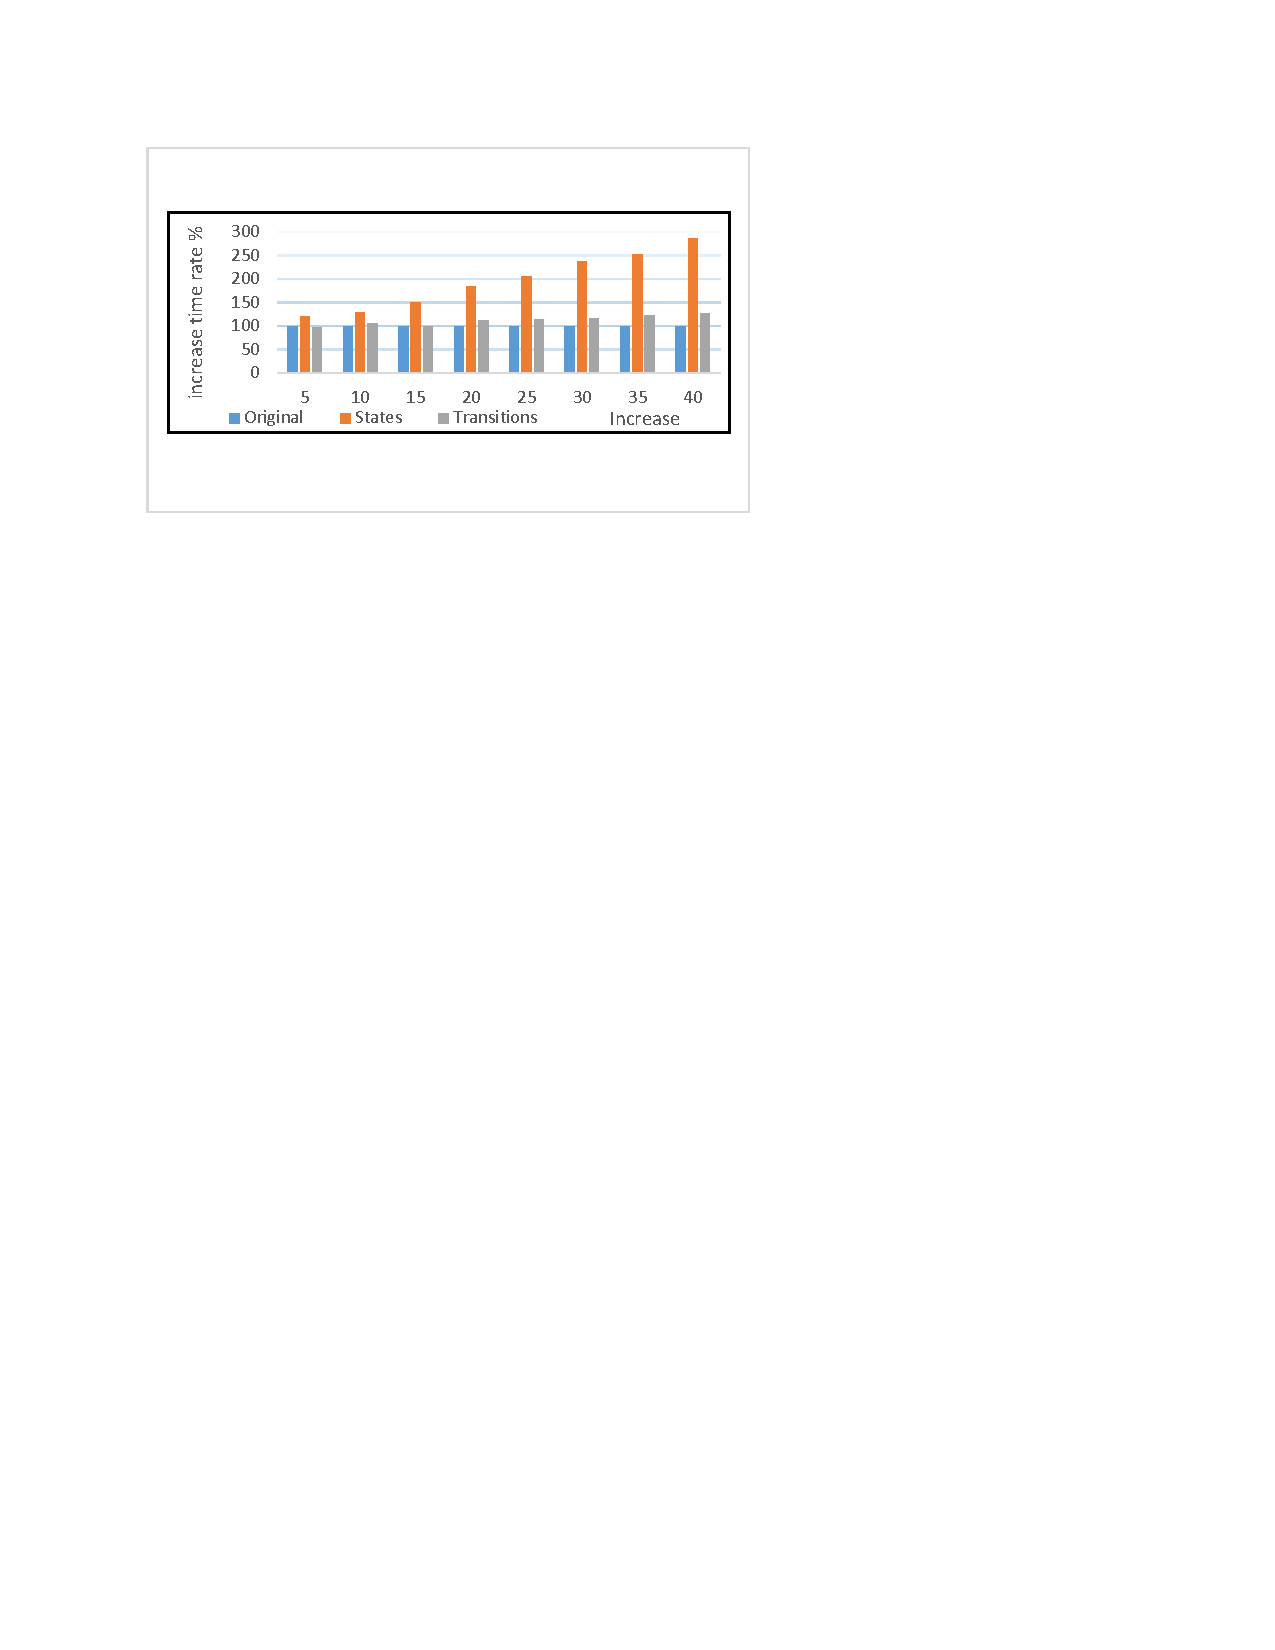
\includegraphics[clip, trim=2.8cm 20.6cm 9cm 3.6cm, width=0.35\textwidth]{figures/graph}
\caption{Performance impact comparison between states and transitions} 
\label{fig:graph}
\end{figure}